\documentclass[12pt,a4paper]{article}
\usepackage[czech]{babel}
\usepackage[T1]{fontenc}
\usepackage[utf8]{inputenc}
\usepackage{lmodern}
\usepackage{graphicx}
\usepackage{listings}
\usepackage{url}
\usepackage{hyperref}
\usepackage{xcolor}
\usepackage{geometry}
\usepackage{dirtree}


\geometry{a4paper, margin=2.5cm}

\lstset{
    basicstyle=\small\ttfamily,
    keywordstyle=\color{blue},
    commentstyle=\color{green!50!black},
    stringstyle=\color{red},
    numbers=left,
    numberstyle=\tiny\color{gray},
    stepnumber=1,
    numbersep=5pt,
    backgroundcolor=\color{white},
    showspaces=false,
    showstringspaces=false,
    showtabs=false,
    frame=single,
    tabsize=4,
    captionpos=b,
    breaklines=true,
    breakatwhitespace=false,
    framexleftmargin=0mm,
    framexrightmargin=0mm,
    framesep=2mm,
    xleftmargin=5mm,
    xrightmargin=0mm,
    language=Python
}

\title{KNN-Math: Rozpoznávání matematických vzorců}
\author{Dokumentace projektu}
\date{\today}

\begin{document}

\maketitle

\tableofcontents
\newpage

\section{Úvod}

Tento dokument popisuje strukturu a implementaci projektu KNN-Math, který se zaměřuje na rozpoznávání matematických vzorců pomocí algoritmu k-nejbližších sousedů (KNN). Systém je navržen pro rozpoznávání jak tištěných, tak off-line ručně psaných matematických výrazů a jejich převod do formátu LaTeX.

\section{Struktura projektu}

Projekt je organizován do modulárního systému, který usnadňuje údržbu a rozšiřitelnost. Hlavní adresářová struktura je následující:



\section{Popis modulů}

\subsection{Modul main.py}

Tento modul slouží jako hlavní vstupní bod aplikace a poskytuje rozhraní příkazové řádky pro různé operace:
\begin{itemize}
    \item Trénování modelu pomocí trénovacích dat
    \item Testování modelu na testovacích datech
    \item Rozpoznávání matematických výrazů v jednotlivých obrázcích
\end{itemize}

\subsection{Modul preprocessing}

Tento modul se stará o přípravu vstupních obrázků pro rozpoznávání:

\begin{itemize}
    \item \textbf{segmentation.py} - Obsahuje funkce pro segmentaci matematických symbolů z celého obrázku, převod obrázků do stupňů šedi, prahování pro oddělení symbolů od pozadí a normalizaci velikosti obrázků na standardní rozměr.
\end{itemize}

\subsection{Modul recognition}

Tento modul implementuje algoritmus rozpoznávání symbolů:

\begin{itemize}
    \item \textbf{knn\_classifier.py} - Implementuje KNN klasifikátor pro rozpoznávání jednotlivých symbolů. Zahrnuje funkce pro trénování modelu, predikci symbolů, ukládání a načítání natrénovaného modelu.
\end{itemize}

\subsection{Modul parsing}

Tento modul převádí rozpoznané symboly do LaTeX formátu:

\begin{itemize}
    \item \textbf{latex\_converter.py} - Obsahuje mapování mezi rozpoznanými symboly a jejich LaTeX reprezentací, a funkci pro sestavení výsledného LaTeX kódu z posloupnosti symbolů.
\end{itemize}

\subsection{Modul utils}

Tento modul poskytuje pomocné funkce:

\begin{itemize}
    \item \textbf{data\_loader.py} - Funkce pro načítání obrázků a popisků z datasetu.
    \item \textbf{evaluation.py} - Funkce pro vyhodnocení přesnosti a výkonnosti modelu.
\end{itemize}

\subsection{Modul config.py}

Konfigurační soubor obsahující globální parametry:

\begin{itemize}
    \item Cesty k adresářům (dataset, modely)
    \item Parametry KNN klasifikátoru (počet sousedů, váhy)
    \item Parametry pro předzpracování obrázků (velikost po normalizaci)
\end{itemize}

\section{Algoritmus rozpoznávání}

Algoritmus rozpoznávání matematických výrazů v aplikaci probíhá v následujících krocích:

\begin{enumerate}
    \item \textbf{Načtení vstupního obrázku} - Obrázek je načten a převeden do stupňů šedi.
    
    \item \textbf{Segmentace symbolů} - Obrázek je prahován pro oddělení symbolů od pozadí. Následně jsou nalezeny kontury jednotlivých symbolů a extrahovány jako samostatné obrázky.
    
    \item \textbf{Předzpracování symbolů} - Každý extrahovaný symbol je normalizován na standardní velikost a provedeny další úpravy pro zvýšení přesnosti rozpoznávání.
    
    \item \textbf{Klasifikace symbolů} - KNN klasifikátor predikuje identitu každého symbolu na základě natrénovaného modelu.
    
    \item \textbf{Konverze do LaTeXu} - Posloupnost rozpoznaných symbolů je převedena do LaTeX formátu, který zachovává matematickou strukturu výrazu.
\end{enumerate}

\section{KNN klasifikátor}

Pro rozpoznávání jednotlivých symbolů je použit algoritmus k-nejbližších sousedů (KNN). Princip tohoto algoritmu je následující:

\begin{itemize}
    \item Každý obrázek je reprezentován jako vektor příznaků (v našem případě jako vektor hodnot pixelů).
    \item Pro klasifikaci nového symbolu je vypočtena vzdálenost mezi jeho vektorem příznaků a vektory všech trénovacích vzorků.
    \item Je vybráno $k$ trénovacích vzorků s nejmenší vzdáleností.
    \item Nový symbol je klasifikován do třídy, která se nejčastěji vyskytuje mezi těmito $k$ nejbližšími sousedy.
\end{itemize}

V implementaci používáme weighted KNN, kde vzdálenější sousedé mají menší vliv na konečnou klasifikaci.

\section{Dataset a trénování}

Pro trénování a testování modelu je použit dataset matematických symbolů. Dataset obsahuje tisíce obrázků v adresáři \texttt{dataset} a soubor \texttt{train\_labels.txt}, který obsahuje mapování mezi názvy souborů a odpovídajícími symboly.

Proces trénování zahrnuje:
\begin{enumerate}
    \item Načtení obrázků a jejich štítků
    \item Předzpracování obrázků (normalizace velikosti, převod do stupňů šedi, atd.)
    \item Extrakce příznaků (v našem případě příznaky jsou přímo hodnoty pixelů)
    \item Trénování KNN klasifikátoru
    \item Uložení natrénovaného modelu pro pozdější použití
\end{enumerate}

\section{Evaluace}  % Testovani
Během rozpoznání může dojít ke dvěma typům errorů: error v rozpoznání symbolu a error v rozpoznání struktury~\ref{img:errors}.
% ===== errors img =====
\begin{figure}[h!]
    \centering
    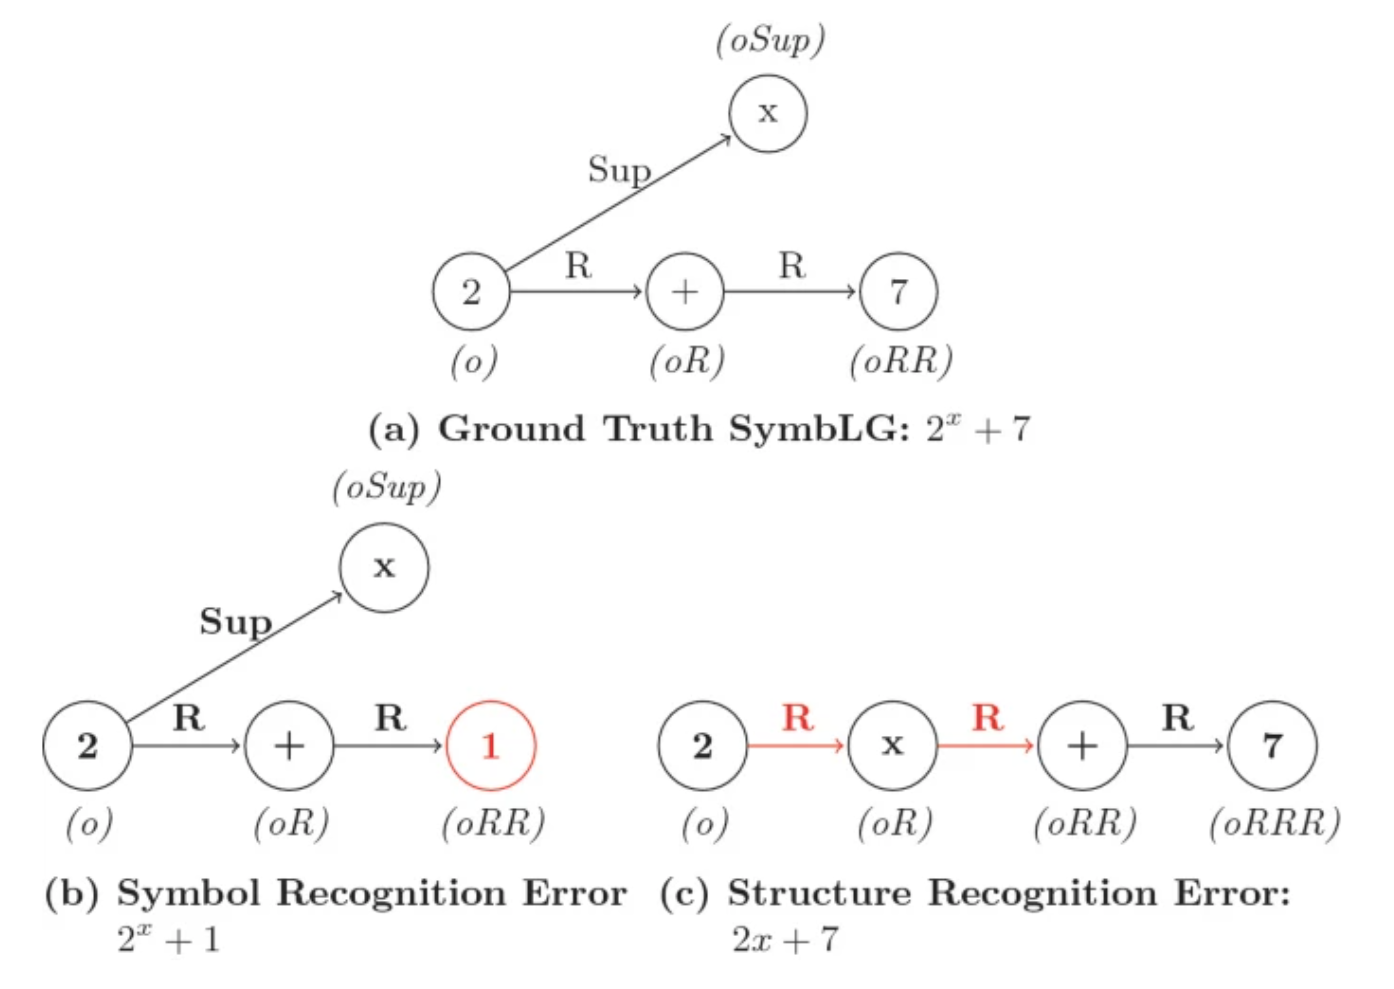
\includegraphics[width=0.8\textwidth]{img/errors.png}
    \caption{Příklady možných chyb při rozpoznávání}
    \label{img:errors}
\end{figure}
 


\section{Použití aplikace}

Aplikaci lze použít několika způsoby:

\subsection{Trénování modelu}

\begin{lstlisting}[language=bash]
python -m app.main --train
\end{lstlisting}

\subsection{Testování modelu}

\begin{lstlisting}[language=bash]
python -m app.main --test
\end{lstlisting}

\subsection{Rozpoznávání matematického výrazu v obrázku}

\begin{lstlisting}[language=bash]
python -m app.main --recognize cesta/k/obrazku.png --output vystup.tex
\end{lstlisting}

\section{Možná rozšíření}

Navržená struktura projektu umožňuje snadné rozšíření o další funkce:

\begin{itemize}
    \item \textbf{Lepší algoritmy segmentace} - Implementace pokročilejších metod pro segmentaci složitějších matematických struktur (zlomky, mocniny, integrály).
    
    \item \textbf{Pokročilejší klasifikátory} - Nahrazení KNN klasifikátoru konvolučními neuronovými sítěmi nebo jinými algoritmy strojového učení.
    
    \item \textbf{Rozpoznávání struktury} - Implementace algoritmů pro rozpoznávání struktury matematických výrazů, nejen jednotlivých symbolů.
    
    \item \textbf{Webové rozhraní} - Vytvoření webového rozhraní pro snadné použití aplikace.
\end{itemize}

\section{Závěr}

Tato dokumentace popisuje strukturu a implementaci projektu KNN-Math. Projekt je navržen modulárně, což umožňuje snadnou údržbu a rozšiřování. Implementovaný systém používá algoritmus k-nejbližších sousedů pro rozpoznávání matematických symbolů a převod do LaTeX formátu.

\end{document} 